
\documentclass{article}
\usepackage[utf8]{inputenc}
\usepackage{graphicx}
\usepackage{float}

\begin{document}

\begin{figure}[H]
\centering
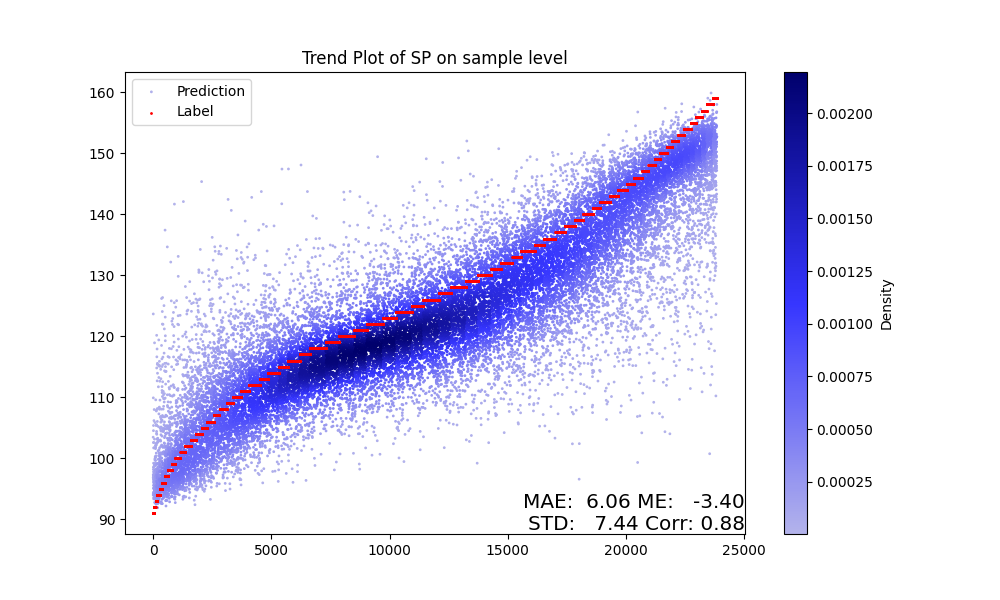
\includegraphics[width=\textwidth]{./Fig/Trend_Plot_SP_on_sample_level.png}
\caption{Trend Plot of SP on sample level.}
\label{fig:image1}
\end{figure}

\begin{figure}[H]
\centering
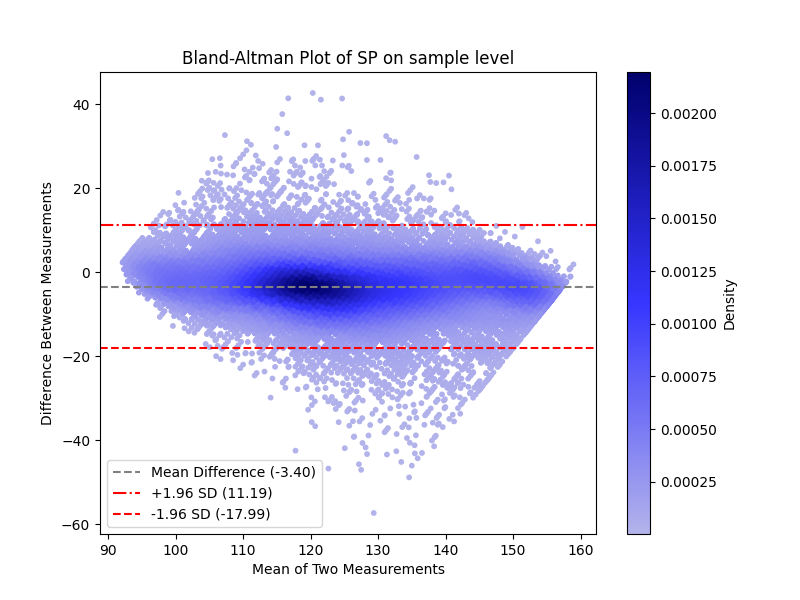
\includegraphics[width=\textwidth]{./Fig/Bland_Altman_Plot_SP_on_sample_level.png}
\caption{Bland-Altman plot of all subjects' SP prediction vs label measurements. Here one dot represents one measurement pair.}
\label{fig:image1}
\end{figure}

\begin{figure}[H]
\centering
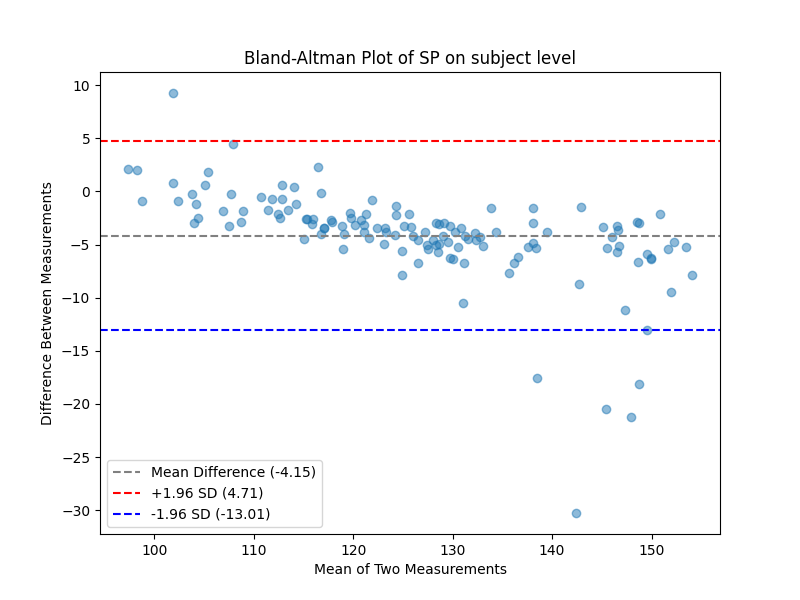
\includegraphics[width=\textwidth]{./Fig/Bland_Altman_Plot_SP_on_subject_level.png}
\caption{Bland-Altman plot of each subject's averaged SP prediction vs label measurements. Here one dot represents one subject.}
\label{fig:image1}
\end{figure}

\begin{figure}[H]
\centering
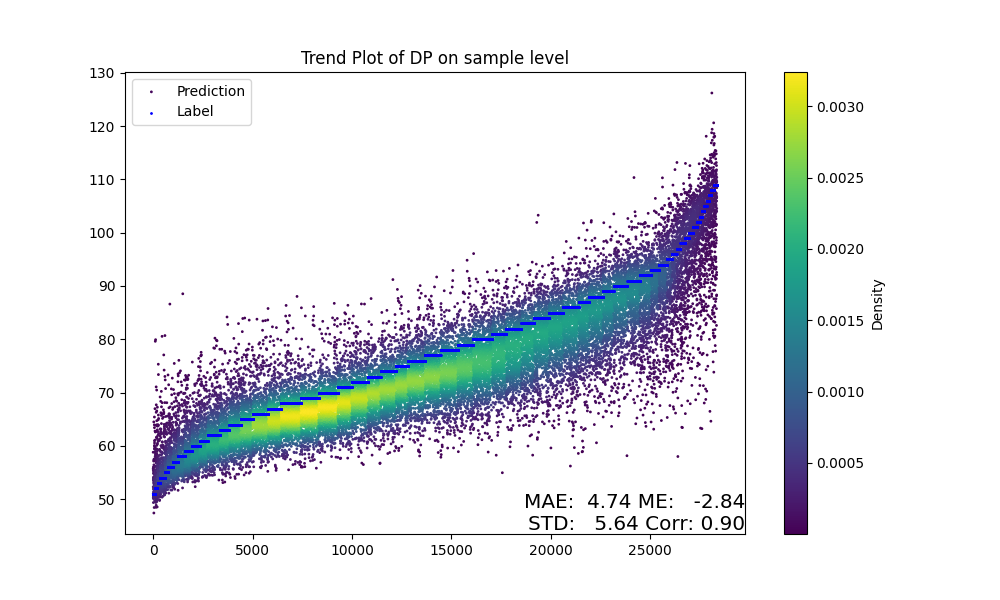
\includegraphics[width=\textwidth]{./Fig/Trend_Plot_DP_on_sample_level.png}
\caption{Trend Plot of DP on sample level.}
\label{fig:image1}
\end{figure}

\begin{figure}[H]
\centering
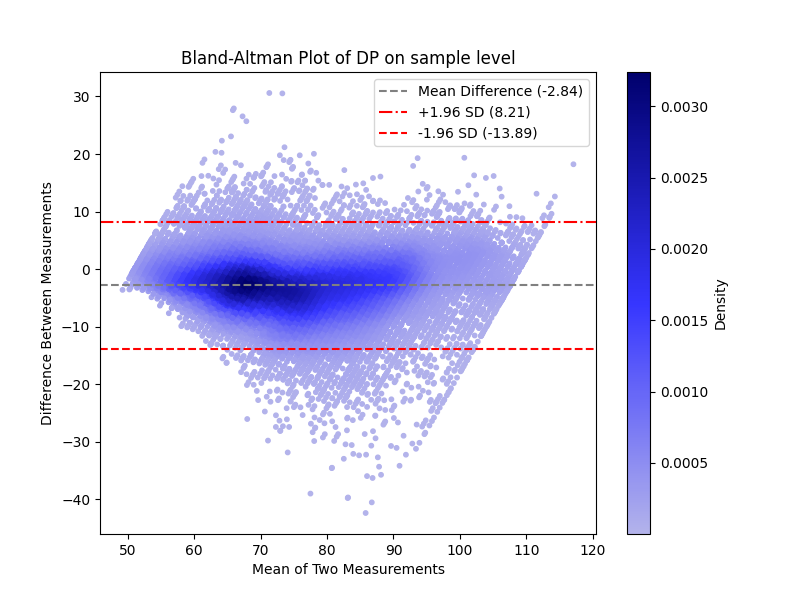
\includegraphics[width=\textwidth]{./Fig/Bland_Altman_Plot_DP_on_sample_level.png}
\caption{Bland-Altman plot of all subjects' DP prediction vs label measurements. Here one dot represents one measurement pair.}
\label{fig:image1}
\end{figure}

\begin{figure}[H]
\centering
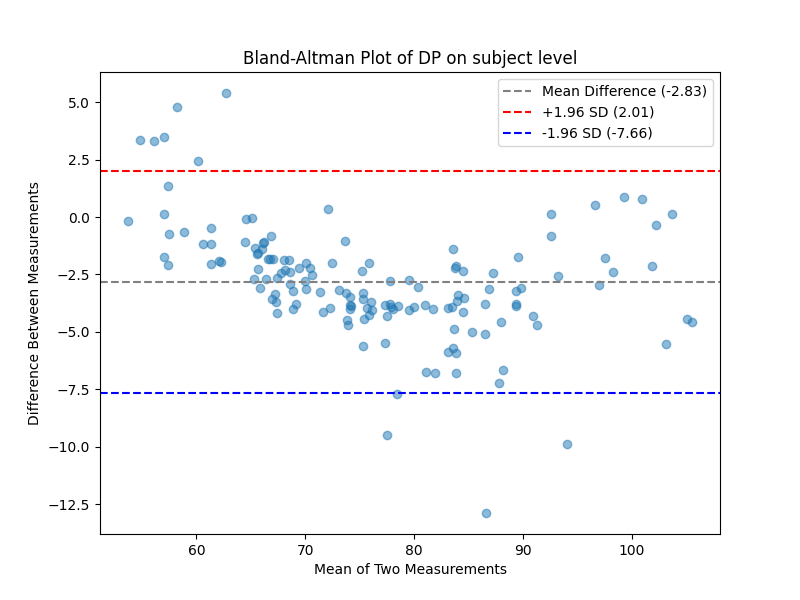
\includegraphics[width=\textwidth]{./Fig/Bland_Altman_Plot_DP_on_subject_level.png}
\caption{Bland-Altman plot of each subject's averaged DP prediction vs label measurements. Here one dot represents one subject.}
\label{fig:image1}
\end{figure}

\begin{figure}[H]
\centering
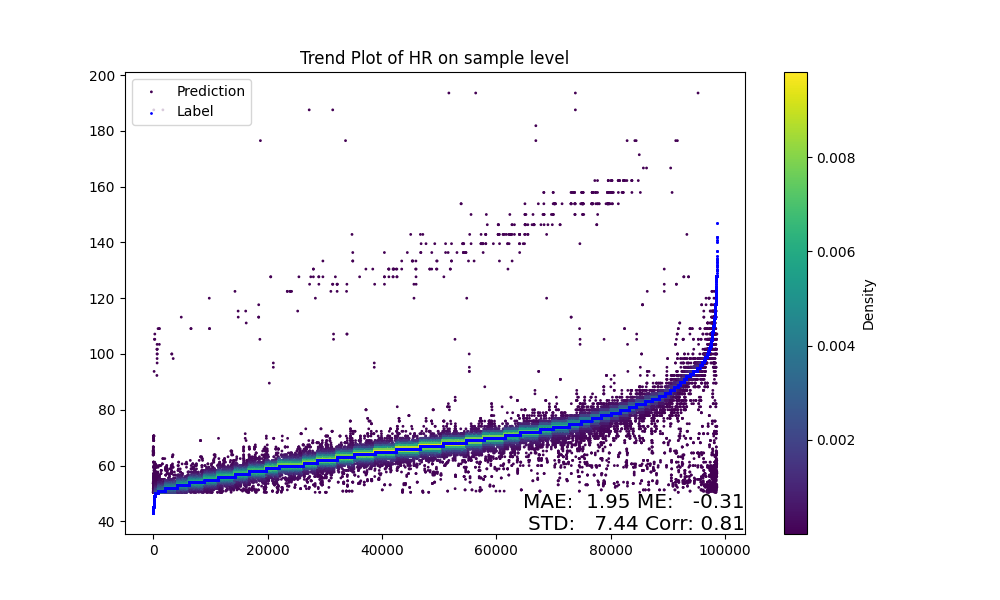
\includegraphics[width=\textwidth]{./Fig/Trend_Plot_HR_on_sample_level.png}
\caption{Trend Plot of HR on sample level.}
\label{fig:image1}
\end{figure}

\begin{figure}[H]
\centering
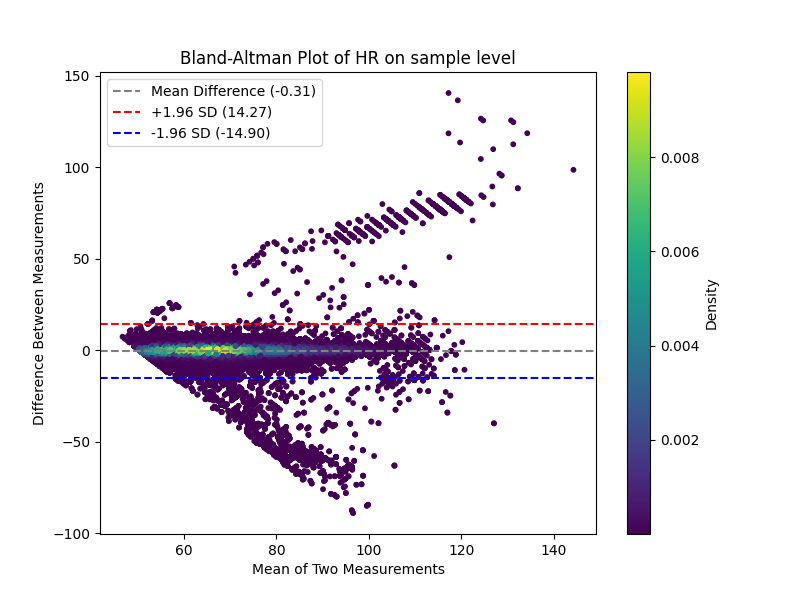
\includegraphics[width=\textwidth]{./Fig/Bland_Altman_Plot_HR_on_sample_level.png}
\caption{Bland-Altman plot of all subjects' HR prediction vs label measurements. Here one dot represents one measurement pair.}
\label{fig:image1}
\end{figure}

\begin{figure}[H]
\centering
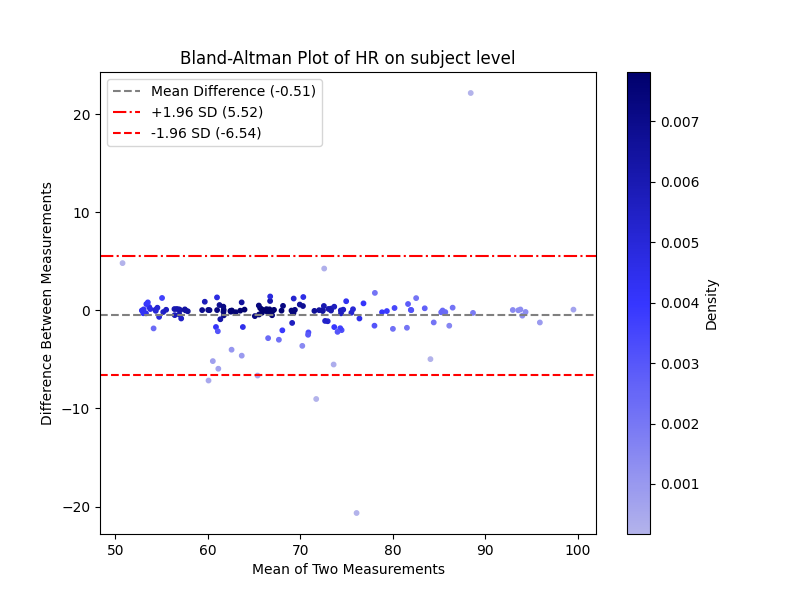
\includegraphics[width=\textwidth]{./Fig/Bland_Altman_Plot_HR_on_subject_level.png}
\caption{Bland-Altman plot of each subject's averaged HR prediction vs label measurements. Here one dot represents one subject.}
\label{fig:image1}
\end{figure}

\begin{figure}[H]
\centering
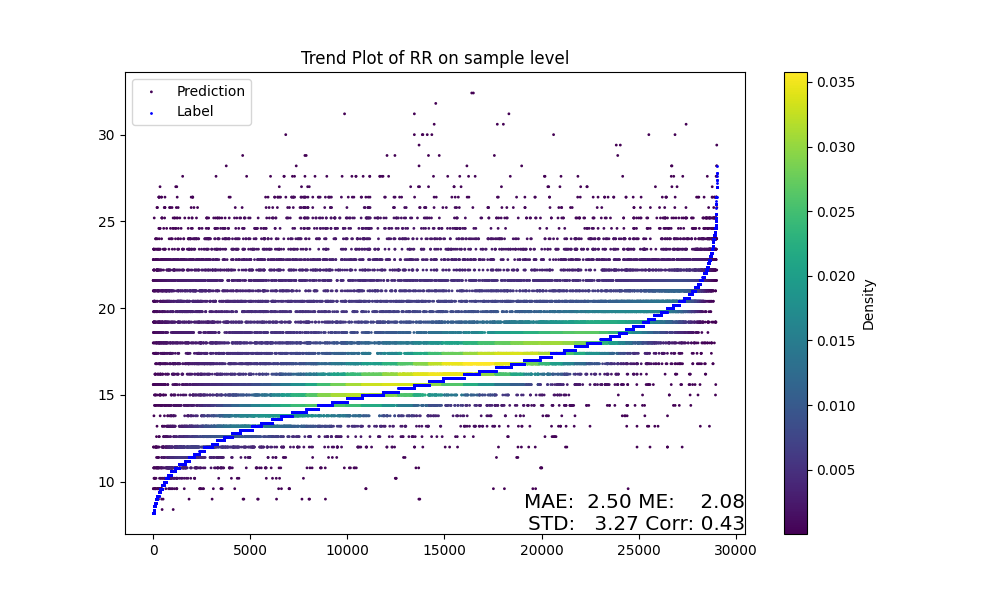
\includegraphics[width=\textwidth]{./Fig/Trend_Plot_RR_on_sample_level.png}
\caption{Trend Plot of RR on sample level.}
\label{fig:image1}
\end{figure}

\begin{figure}[H]
\centering
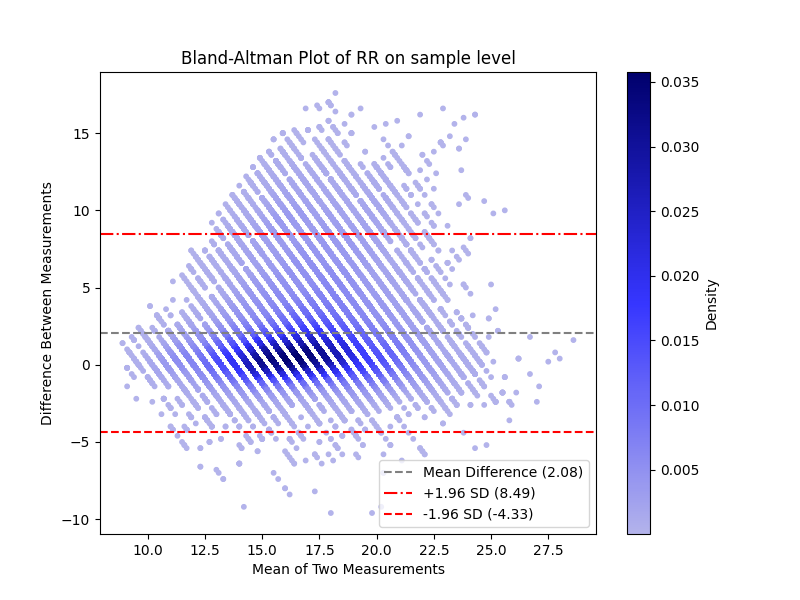
\includegraphics[width=\textwidth]{./Fig/Bland_Altman_Plot_RR_on_sample_level.png}
\caption{Bland-Altman plot of all subjects' RR prediction vs label measurements. Here one dot represents one measurement pair.}
\label{fig:image1}
\end{figure}

\begin{figure}[H]
\centering
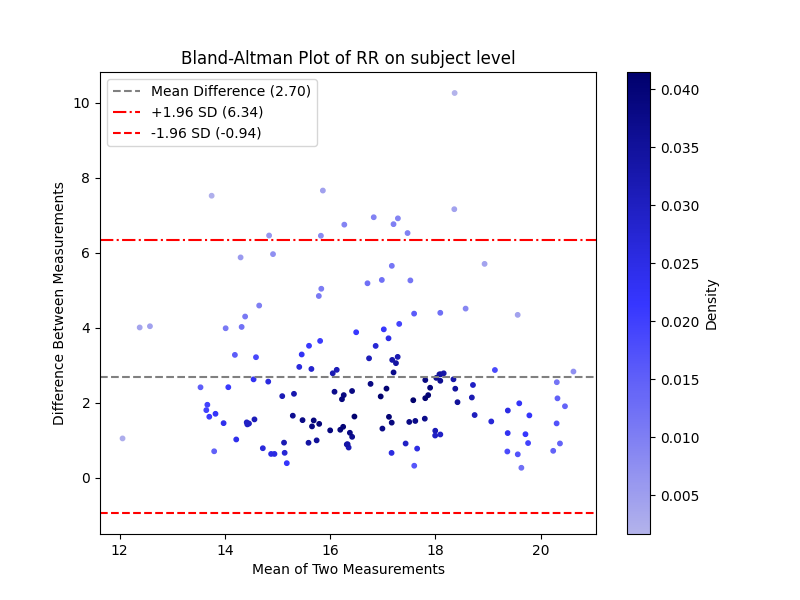
\includegraphics[width=\textwidth]{./Fig/Bland_Altman_Plot_RR_on_subject_level.png}
\caption{Bland-Altman plot of each subject's averaged RR prediction vs label measurements. Here one dot represents one subject.}
\label{fig:image1}
\end{figure}


\begin{figure}[H]
\centering
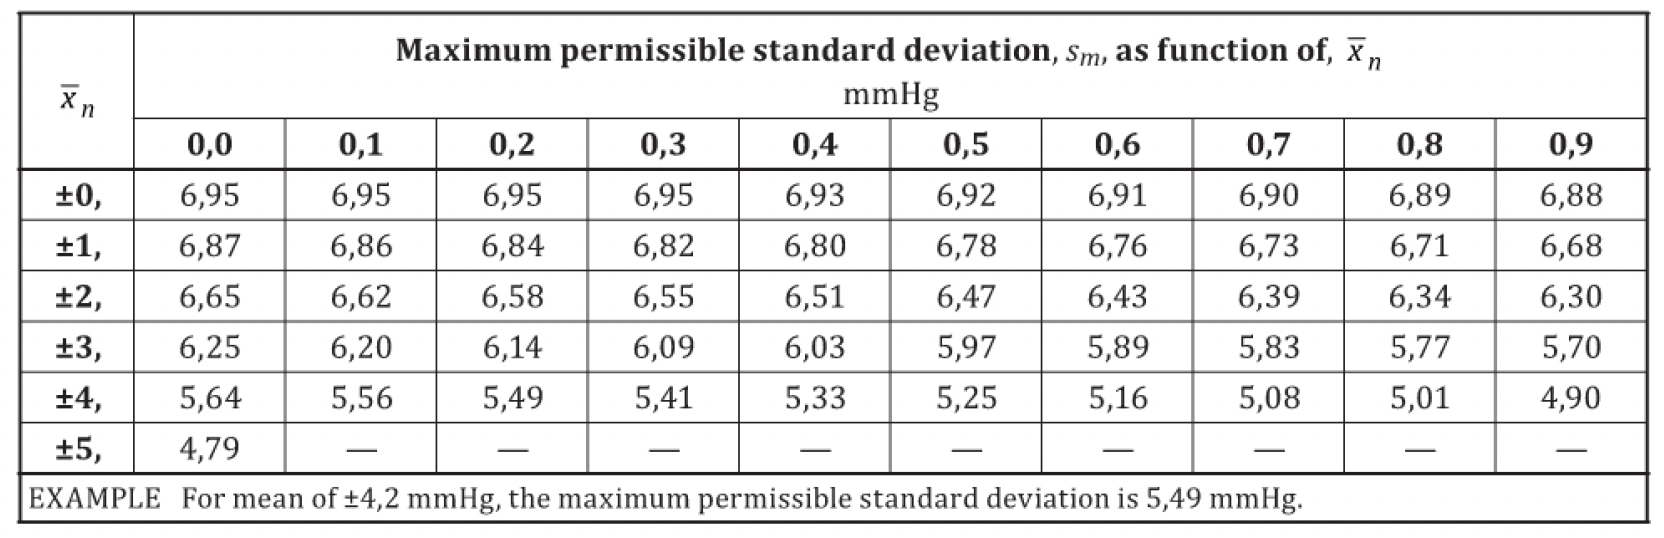
\includegraphics[width=0.8\textwidth]{./Fig/ME_STD_Correspond.png}
\caption{Averaged subject data acceptance in mmHg}
\label{ME_STD}
\end{figure}

\begin{table}[h!]
\centering
\begin{tabular}{|c|c|c|c|c|c|}
\hline
Vital Signal & ME & MAE & SD & Correlation & Whether meet the requirement\\ \hline


SP on sample level & -3.40 & 6.06 & 7.44 & 0.88 & Yes \\ \hline

SP on subject level & -4.15 & 4.52 & 4.52 & 0.97 & Yes \\ \hline

DP on sample level & -2.84 & 4.74 & 5.64 & 0.90 & Yes \\ \hline

DP on subject level & -2.83 & 3.20 & 2.47 & 0.98 & Yes \\ \hline

HR on sample level & -0.31 & 1.95 & 7.44 & 0.81 & Yes \\ \hline

HR on subject level & -0.51 & 1.27 & 3.08 & 0.96 & Yes \\ \hline

RR on sample level & 2.08 & 2.50 & 3.27 & 0.43 & Yes \\ \hline

RR on subject level & 2.70 & 2.70 & 1.86 & 0.61 & Yes \\ \hline


\end{tabular}
\caption{Prediction Results}
\label{tab:metrics}
\end{table}

\end{document}
